% !TeX program = pdflatex
% !BIB program = bibtex
% ICASSP 2027 submission source built from the official ICASSP 2027 kit.
% Official archive:
% https://cmsworkshops.com/ICASSP2027/papers/PaperFormat/ICASSP2027_Paper_Templates.zip
% Official spconf.sty and IEEEbib.bst are included unchanged.
% Release package and scientific manuscript body: v110 (2026-09-04).
% --------------------------------------------------------------------------
\documentclass{article}
\usepackage{spconf,amsmath,amssymb,graphicx,booktabs,array,hyperref}
\hypersetup{hidelinks}
\name{Seunghun Oh$^{1}$\qquad Unsang Park$^{2}$}
\address{$^{1}$Department of Artificial Intelligence, Sogang University, Seoul, Republic of Korea\\
  $^{2}$Department of Computer Science and Engineering, Sogang University, Seoul, Republic of Korea}
\let\srvrabstract\abstract
\let\endsrvrabstract\endabstract
\renewenvironment{abstract}{\maketitle\srvrabstract}{\endsrvrabstract}

\begin{document}
\ninept
% !TeX root = Template.tex
% Manuscript body included by Template.tex.

\title{Speech as Pointer and Distractor in CMTB: A Factorial Diagnosis of Frozen AV-LLMs}

\begin{abstract}
Instructional speech can serve two conflicting roles: its occurrence points to a video moment, while its content may describe an action from another moment. We study this conflict on the Cross-Modal Temporal Binding (CMTB) benchmark by separating the timing reference from the waveform available when a model answers. Across the three primary numeric-interface AV-LLMs, supplying timing changes waveform audio's effect by $17.2$--$27.1$ percentage points, making it less useful or sometimes harmful. With the reference fixed, 19 of Qwen3's 21 correct-to-wrong transitions select the narrated distractor. Speech-Referenced Visual Re-query (SRVR) uses an automatically detected speech interval to revisit the relevant visual evidence and answers without waveform audio. Timing-displacement, matched-frame, and black-video controls show that improvement depends on the correct visual moment. The effect remains model-, interface-, task-, and benchmark-dependent.
\end{abstract}

\begin{keywords}
Audio-visual language models, cross-modal arbitration, hallucination, speech timing, temporal binding
\end{keywords}

\section{Introduction}
\label{sec:introduction}

Instructional narration can preview or recap rather than caption the concurrent action. In SVHalluc's Cross-Modal Temporal Binding (CMTB) task, a model must select what is visibly happening when speech occurs from three choices: the current action $y$, an off-time action named by narration $d_n$, and an unrelated action $d_u$~\cite{zhang2026svhalluc}. Before the first model evaluation, we partitioned the official 339 CMTB items into a fixed, video-disjoint Dev-48 and locked evaluation split CMTB-291; prompt wording and VAD threshold were chosen on Dev-48 alone, and every headline CMTB result uses CMTB-291. Figure~\ref{fig:example} shows one locked item: the video shows cubed bread being added, while speech describes mixing milk and egg; Raw AV selects the narrated choice.

SVHalluc reports CMTB failure, transcript degradation, and speech-time localization separately. It does not cross answering-time waveform audio with externally held timing on the same items, estimate their interaction, or test whether induced errors transition selectively to the narrated option. We perform that behavioral decomposition, then use displacement and black-video controls to test time-specific visual-evidence use. The contribution is neither a new VAD algorithm nor the expected gain from exposing its interval, but the decomposition: fixed occurrence changes the waveform's marginal value, and added losses flow selectively toward the narrated option.

CMTB defines the requested moment by speech occurrence, so exposing that occurrence is not itself a localization algorithm. The question is whether frozen models execute this stated lookup when the visual evidence is already present. Five controls isolate the gap: numeric references retain the full video, an exact same-frame-count control fixes how much video is seen, equal-duration random intervals test shortening, displacement tests whether accuracy follows the referenced moment, and black video tests whether timestamps and options suffice without visual evidence. A large correction under such a minimal probe is evidence for a behavioral current-time binding gap rather than for a sophisticated localizer.

Our contributions are:
\begin{itemize}
\setlength{\itemsep}{0pt}\setlength{\parsep}{0pt}\setlength{\parskip}{0pt}\setlength{\topsep}{2pt}
\item \textbf{Factorial diagnosis:} a locked-split Audio$\times$Reference interaction in three systems on probability and logistic scales.
\item \textbf{Behavioral isolation:} selective shifts toward $d_n$, plus prompt, location, frame-budget, visual-evidence, speech-waveform, and content controls.
\item \textbf{Scoped correction:} the speech-time reference raises the audio-free accuracy point estimate in all six reported configurations; model and task nulls bound its scope.
\end{itemize}

\begin{figure*}[t]
\centering
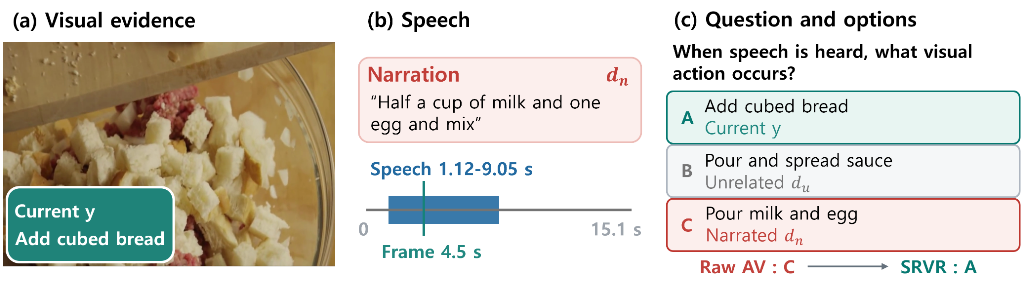
\includegraphics[width=\textwidth]{figures/figure1.pdf}
\caption{One locked CMTB item. Speech occurrence identifies the requested time, but its content names an off-time action. Qwen3 Raw AV selects the narrated option $d_n$; supplying the automatic speech interval and answering without audio recovers the current visual answer $y$. The item is illustrative, not a prevalence estimate.}
\label{fig:example}
\end{figure*}

\section{Related Work}
\label{sec:related-work}

Classical voice activity detection (VAD) estimates speech presence from acoustic statistics~\cite{sohn1999vad}, while self-supervised audio--visual synchronization learns temporal correspondence between acoustic and visual streams~\cite{korbar2018avsync}. Here VAD externalizes occurrence only; the diagnosed failure is downstream evidence binding when speech semantics name another event. Visual narration detection asks whether narrated content is depicted~\cite{ashutosh2023wys2}; cross-modal studies evaluate temporal, semantic, premise, and decision-level conflict~\cite{kim2024avhbench,zhou2026avsyncbench,chen2026avid,nguyenquang2026senseswide}. Unlike synchronized semantic conflicts~\cite{sudheer2026prior}, ours uses truthful off-time narration whose occurrence defines the requested moment. Temporal-grounding methods localize query-described events through learned frame selection, visual markers, or generalist span prediction~\cite{du2026mllmsknowwhen,wang2026videoitg,fang2026markit,zhang2026timelens}; their query normally names the target event. Read-then-regenerate approaches surface a model's own temporal signal and re-query the recovered interval~\cite{du2026mllmsknowwhen}, but we measure the Audio$\times$Reference non-additivity after that interval is supplied. ChronusOmni applies temporal RL to timestamped audio-visual representations~\cite{chen2025chronusomni}; AVCD and related methods modify internal evidence or decoding~\cite{leng2024vcd,jung2025avcd,fan2026stear,wu2026season}; and instruction-aware gating addresses modality arbitration~\cite{ding2026unimvu}. Narration-to-video alignment~\cite{mavroudi2023htstep} instead aligns narration to the event it describes.

\section{Method}
\label{sec:method}

\subsection{Speech-Referenced Visual Re-query (SRVR)}

Let frozen model $M$ receive video $V$, audio $A$, and the unchanged multiple-choice question $q$. Silero-VAD 6.2.1 processes 16-kHz audio with threshold .5, minimum speech/silence durations 250/100 ms, and 30-ms padding~\cite{silero_vad621}. The first detected start and last detected end form the speech envelope $\hat I_s$. This extraction is answer-blind: it uses no question, option, action label, prediction, correctness, or manual timestamp.

SRVR then exposes visual evidence at $\hat I_s$ through the model's native interface, disables answering-time audio, and asks the unchanged question $q$ with deterministic decoding. For Qwen2.5-Omni-7B and Qwen3-Omni-30B-A3B-Instruct~\cite{xu2025qwen25omni,xu2025qwen3omni}, the complete video is retained and the exact prefix is: ``The relevant speech activity occurs from START to END seconds. Answer using only the visual action during that interval. Do not infer or use transcript content.'' Qwen samples at 2 fps; the official ChronusOmni checkpoint retains its 64-frame timestamp construction and the same prefix. For video-SALMONN-2~\cite{tang2025videosalmonn2} and VideoLLaMA2.1-7B-AV~\cite{cheng2024videollama2}, the unchanged question receives $V[\hat I_s]$ with audio disabled through the native localized interface; their loaders use approximately 1 fps and 8 frames, respectively. Numeric and localized interfaces are analyzed separately, never pooled. To cross interface with architecture, Qwen2.5/3, ChronusOmni, and Phi-4-multimodal-instruct also answer from the VAD crop, with the waveform cropped to the same window in the audio-on twin. ChronusOmni and Phi-4 retain their official frame counts and re-base frame times to the crop origin, so no numeric reference survives; numeric-interface Phi-4 instead reads 32 timestamp-labeled full-video frames.

\begin{table*}[t]
\centering
\caption{Locked CMTB-291 accuracy (\%). Waveform denotes answering-time audio; timing is derived beforehand. The first three rows define the central nine-test reporting family; the rest are scope checks. $\Delta_{int}$ uses unrounded proportions. $\dagger$: restricting to the $N=231$ items parsed in all four cells gives $+6.1$ pp $[+0.4,+11.7]$ and no negative reversal.}
\label{tab:main}
\begin{tabular}{@{}llrrrrr@{}}
\toprule
& & \multicolumn{2}{c}{No reference} & \multicolumn{2}{c}{Reference} & \\
\cmidrule(lr){3-4}\cmidrule(lr){5-6}
Model & Interface & Waveform off & Waveform on & Waveform off & Waveform on & $\Delta_{int}$ \\
\midrule
Qwen3-Omni & numeric & 47.1 & 60.8 & \textbf{90.0} & 86.6 & $-17.2$ \\
Qwen2.5-Omni & numeric & 46.7 & 52.9 & \textbf{74.2} & 59.1 & $-21.3$ \\
ChronusOmni & numeric & 47.1 & 68.4 & \textbf{86.6} & 80.8 & $-27.1$ \\
Phi-4-multimodal & numeric & 45.4 & 48.1 & 57.4 & 61.5 & $+1.4$ \\
video-SALMONN-2 & localized & 47.4 & 45.7 & \textbf{81.4} & 80.1 & $+0.3$ \\
VideoLLaMA2.1$^\dagger$ & localized & 51.2 & 41.2 & \textbf{77.3} & 67.7 & $+0.3$ \\
\bottomrule
\end{tabular}

\end{table*}

\subsection{Factorial and controls}

For paired correctness $Y_{pa}$, $p$ indicates whether the external temporal reference is present and $a$ indicates whether answering-time waveform audio is present. The reference is derived from audio once, before answering, so the audio factor is the marginal effect of the waveform given externalized timing. The four same-item factorial cells are Video-only ($Y_{00}$), Raw AV ($Y_{01}$), SRVR ($Y_{10}$), and Reference+Audio ($Y_{11}$); Video-only is a counterfactual that removes the speech-occurrence cue, not a competing system. The central post-specified interaction is
\begin{equation}
\Delta_{int}=(Y_{11}-Y_{10})-(Y_{01}-Y_{00}).
\end{equation}
Because the reference is deterministically extracted from $A$, $\Delta_{int}$ measures input-level behavioral non-additivity rather than independent internal causal pathways.

The post-specified contrast uses four independently frozen same-item conditions; no cell was rerun or retuned. Later follow-ups were frozen before inference but reuse the evaluation split. The prompt follow-up compares the full prefix above with the exact bare prefix ``Speech occurs from START to END seconds.'' and the no-time instruction ``Focus on the relevant moment in the video. Answer using only the visual action at that moment. Do not infer or use transcript content.'' A same-model Qwen2.5 speech-waveform factorial crosses reference status with audio off, a time-reversed Demucs vocal waveform~\cite{rouard2023htdemucs}, or original audio on one fixed, prediction-blind media- and processor-QC subset ($N=249$). Reversed vocals are RMS-matched within VAD segments and recombined with residual background.

Temporal specificity moves only the two timestamp values from $\hat I_s$ toward a farthest equal-duration interval at $\alpha=0,.25,.5,.75,1$, holding video, audio absence, question, options, checkpoint, and decoder fixed. The matched-content study instead keeps full-video SRVR and audio off, then appends ``Automatic narration transcript (provided for a controlled diagnostic): TEXT.'' Original automatic-speech-recognition (ASR) text is compared with length-matched unrelated or current-compatible donor ASR; 244 of 291 items admit both donors. The latter shares a content token with the correct option and none with either distractor, so the answer label enters stimulus construction and the frozen endpoint is $d_n$ choice rate. Equal-duration random intervals, cyclic option rotation, and exact eight-frame InternVL2.5 sampling~\cite{chen2024internvl25} provide complementary controls. Black-video sensitivity substitutes a duration-matched silent clip while holding reference, prompt, options, parser, and decoding fixed. Qwen2.5 VAD-threshold sensitivity holds all other settings fixed. Detector sensitivity uses frozen Systran/faster-Whisper-small.en~\cite{radford2023whisper} (beam 5, temperature 0, VAD filtering off) and spans its first to last decoded segment.

\begin{figure*}[t]
\centering
% \includegraphics[width=\textwidth]{figures/interaction_role_displacement.pdf}
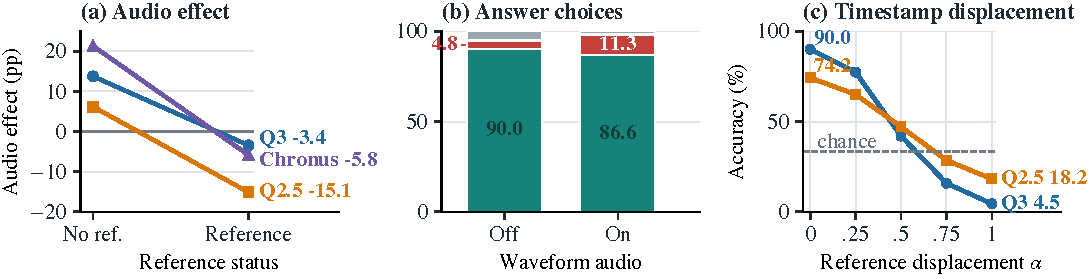
\includegraphics[width=\textwidth]{figures/fig2_balanced_preview.pdf}
\caption{The three central results. (a) An external speech-occurrence reference shifts audio's effect toward negative. (b) With it fixed, Qwen3 current/narrated/role-identified-unrelated/residual counts change from 262/14/0/15 to 252/33/1/5; gray combines no-narrated-role, ambiguous, and parse-failure cases. (c) Moving only the two timestamps away from speech monotonically reduces accuracy.}
\label{fig:quantitative-results}
\end{figure*}

CMTB-291 contains one item from each of 291 source videos, so item and video clusters coincide. Percentile CIs use 20,000 paired source-video bootstrap draws; simple effects use exact McNemar tests. Binomial generalized estimating equations (GEE) cluster the four repeated cells by source-video ID, with an exchangeable working correlation and robust sandwich SE. The central nine-test Holm family covers the three numeric-interface systems available when it was fixed: three interactions and six simple effects. It does not correct the earlier selection of this post-specified contrast. Later Phi-4 and localized-interface cells are scope checks; separate follow-up families cover two bare-timestamp interactions, four localized-interface interactions, and two content-swap contrasts. A conservative sensitivity additionally applies Holm across all six Table~\ref{tab:main} logistic-GEE interaction tests.

\section{Results}
\label{sec:results}

\subsection{Factorial diagnosis}

Audio's marginal effect changes from $+6.2/+13.7/+21.3$ pp without a reference to $-15.1/-3.4/-5.8$ pp with one for Qwen2.5, Qwen3, and ChronusOmni (Fig.~\ref{fig:quantitative-results}a). The interaction CIs are $[-27.8,-14.8]$, $[-23.7,-10.7]$, and $[-34.0,-20.3]$; logistic-GEE ratios of audio odds ratios are .39/.41/.27, all Holm-significant. The three primary interactions also survive a six-interaction Holm sensitivity (largest adjusted $p=4.95\!\times\!10^{-5}$); the three additional Table~\ref{tab:main} interactions do not. Persistence on the logistic scale shows that the interaction is not confined to the probability scale or its ceiling. The Qwen2.5 no-reference benefit and Qwen3 reference-conditioned loss do not survive correction, so interaction---rather than significant help and harm in every model---is the claim. A frozen no-time visual instruction remains at 45.0/46.7\% (Qwen2.5/3), whereas bare timestamps yield $-23.0/-20.6$ pp interactions (Table~\ref{tab:controls}; Holm $p<10^{-8}$), excluding generic visual-focus and anti-transcript wording as necessary causes.

Errors move in the predicted direction. One prediction-blind annotator reviewed the 184-item union of Qwen reference-condition errors. A second independently relabeled a fixed random 100 (78\% agreement, $\kappa=.71$); the 22 disagreements were adjudicated. Of the 184 items, 117 admit determinate option roles; Qwen estimates use all 291 items and set unresolved role indicators to zero. Qwen3 audio causes 21 correct-to-wrong and 11 wrong-to-correct transitions (262$\to$252 correct); 19 of the 21 losses select $d_n$. Direct $y\!\leftrightarrow\!d_n$ transitions are 19 versus one (exact $p=4.0\times10^{-5}$). Marginal current/$d_n$/identified-$d_u$/residual counts change from 262/14/0/15 to 252/33/1/5 (Fig.~\ref{fig:quantitative-results}b); residual combines no-narrated-role, ambiguous, and parse-failure cases. The marginal $d_n$ share rises 6.5 pp, and net direct $y\!\leftrightarrow\!d_n$ flow is 6.2 pp. Qwen2.5's full-denominator $(\Delta d_n-\Delta d_u)$ increase is $+13.4$ pp; assigning its six unmapped audio-on errors adversarially still leaves $+11.3$ pp. Matched content swap moves choices conversely in Qwen3 and directionally in Qwen2.5 (Table~\ref{tab:controls}); because donor text can cue answer tokens, we interpret this as narration-associated rather than lexical-only evidence.

\begin{table*}[t]
\centering
\caption{Controls in factorial, temporal/visual, and narration/scope blocks. Q2.5/Q3/VL2.1 denote Qwen2.5/Qwen3/VideoLLaMA2.1; $N=291$ unless noted. All were frozen pre-inference and output-blind except label-informed content swap; bare/localized/content rows are Holm-controlled follow-ups. CIs use paired source-video bootstrap.}
\label{tab:controls}
\setlength{\tabcolsep}{2.0pt}
\renewcommand{\arraystretch}{0.86}
\begin{tabular}{@{}>{\raggedright\arraybackslash}p{0.24\textwidth}>{\raggedright\arraybackslash}p{0.23\textwidth}>{\raggedright\arraybackslash}p{0.49\textwidth}@{}}
\toprule
Test (model; $N$) & Frozen contrast & Result [95\% CI] (pp unless shown) \\
\midrule
Bare timestamp (Q2.5/Q3) & Full prompt $\to$ bare; full video & $\Delta_{int}$: $-23.0\,[-29.6,-16.8]$; $-20.6\,[-27.1,-14.1]$ \\
Localized 2$\times$2 (Q2.5/Q3/Chronus/Phi-4) & VAD crop; cropped audio in $a=1$ & $\Delta_{int}$: $-23.4\,[-30.6,-16.5]$; $-18.9\,[-25.4,-12.4]$; $-29.6\,[-36.4,-22.3]$; $-7.2\,[-12.7,-1.7]$ \\
\midrule
Displacement (Q3/Q2.5) & Speech time $\to$ farthest equal-duration time ($\alpha:0\to1$) & $90.0\to4.5\%$; $74.2\to18.2\%$ \\
Random crop (SALMONN-2; $N=194$) & Random $\to$ speech; matched duration, no overlap & $18.6\to80.9\%$; $+62.4\,[+55.5,+69.1]$ \\
Eight frames (InternVL) & Uniform $\to$ speech-time sampling & $49.1\to83.8\%$; $+34.7\,[+29.2,+40.2]$ \\
Black video (Q2.5/Q3) & Real $\to$ duration-matched black & $74.2\to32.6\%$; $-41.6\,[-48.1,-35.1]$\newline $90.0\to34.7\%$; $-55.3\,[-61.5,-49.1]$ \\
Rotation (SALMONN-2) & Original $\to$ cyclic option order & $81.4\to82.1\%$, $p=.85$ \\
\midrule
Content swap (Q3/Q2.5; $N=244$) & Original/unrelated/compatible ASR; endpoint $d_n$ & Q3: $14.3/6.6/3.7\%$; compatible$-$unrelated: Q3 $-2.9\,[-5.3,-0.8]$; Q2.5 $-2.1\,[-4.9,+0.8]$ \\
CrossTask~\cite{zhukov2019crosstask} (Q2.5/VL2.1; $N=132$) & No ref.$\to$ref.; 18 tasks, one $\geq80\%$-overlap step + two alternatives & Q2.5: $39.4\to54.5\%$; $+15.2\,[+6.1,+24.2]$\newline VL2.1: $46.2\to72.7\%$; $+26.5\,[+16.7,+36.4]$ \\
TA/TF boundary ($N=570$) & Raw AV $\to$ localized speech-time support & $42.5\to43.7\%$; $+1.2\,[-1.6,+4.0]$, $p=.46$ \\
\bottomrule
\end{tabular}

\end{table*}

\subsection{Speech front end and waveform}

The reference contains a median four speech islands (IQR 2--6) and spans 11.96 s (8.33--16.75), or 45.0\% (40.0--51.0) of video. VAD thresholds .3/.5/.7 yield Qwen2.5 accuracies 72.2/74.2/72.5\%; a frozen faster-Whisper envelope reaches 70.4\%. On the fixed $N=249$ waveform subset, reversed vocals yield $\Delta_{int}=-17.3$ pp (CI $[-22.9,-11.6]$), versus $-20.9$ $[-28.1,-13.7]$ for original audio; their exploratory difference is $-3.6$ $[-9.6,+2.8]$ pp ($p=.305$). Exploratory direct $y\to d_n:d_n\to y$ transitions are 9:1 for off$\to$reversed and 34:1 for off$\to$original (five audio-on errors per arm are unmapped). Most non-additivity survives reversal; direct asymmetry is greater for original audio, but the interaction difference is nonsignificant.

\subsection{Stress tests and scope}

Displacement drives both models below chance; matched-random intervals fail, the gain persists at eight frames, and black video falls to near chance (Fig.~\ref{fig:quantitative-results}c; Table~\ref{tab:controls}). The correction therefore requires visual evidence at the referenced moment, not generic prompting, shortening, extra frames, or fixed option order.

Breadth is mixed. Qwen2.5, Qwen3, and Chronus reverse under both interfaces; Phi-4-multimodal~\cite{microsoft2025phi4mini} reverses only under localized input, while video-SALMONN-2 and VideoLLaMA2.1 show no negative interaction. Their references raise audio-free accuracy from 47.4 to 81.4\% and 51.2 to 77.3\%. VideoLLaMA2.1's audio-on penalties reflect 36/40 parse failures; common-parse $\Delta_{int}=+6.1$ pp. Separately, the four localized follow-up interactions are negative and survive their Holm family; different frame budgets preclude architectural attribution. The reference raises the audio-free accuracy point estimate in all six configurations (57.4--90.0\%; five reach at least 74.2\%).

\section{Discussion and Limitations}
\label{sec:discussion}

\textbf{Evidence and behavioral scope.} The independently frozen cells support a central post-specified analysis, not a preregistered confirmation; same-split follow-ups are secondary, CrossTask is external, and the rest are sensitivities. The factorial identifies input-level non-additivity and the option audit its direction, not an internal circuit. Reversal changes naturalness and text can expose answer tokens, so we claim \emph{narration-associated pressure}, not a lexical-only cause.

\textbf{Interaction composition.} The estimand need not decompose identically across models: Qwen2.5 shows the largest reference-conditioned loss ($-15.1$ pp), whereas Qwen3/Chronus are driven more by positive no-reference contributions ($+13.7/+21.3$ pp) disappearing after occurrence is externalized. Thus $\Delta_{int}$ is reference-dependent audio value, not uniform semantic-harm magnitude.

\textbf{Benchmark and temporal boundary.} The interaction is established only within CMTB. The controls verify referenced visual-input use, not persistence beyond multiple-choice answers. CMTB lacks current- and narrated-action spans; oracle bounds and source-independent replication require new annotation.

\textbf{Deployment boundary.} The Temporal Alignment/Temporal Forecasting (TA/TF) null ($+1.2$ pp, $p=.46$) limits SRVR to questions about visual state at speech occurrence, not temporal reasoning generally.

\section{Reproducibility}
\label{sec:reproducibility}

The video-disjoint partition covers Dev-48 and CMTB-291. Public checkpoints use documented interfaces. Decoding is greedy (32 new tokens; Phi-4: 16); the parser takes the first answer-marked or standalone A/B/C and otherwise scores wrong. VideoLLaMA2.1 parse failures for $Y_{00}/Y_{01}/Y_{10}/Y_{11}$ are 0/36/0/40. Waveform analysis uses a prediction-blind media/processor QC subset (269 successful transforms; $N=249$); other fixed subset sizes for random-interval/content-swap/CrossTask are 194/244/132. CMTB follow-ups were frozen pre-inference but reuse CMTB-291 and were observation-motivated. CrossTask tests external reference utility, not interaction replication. Role labels never enter model input; label-informed content swap evaluates $d_n$, not accuracy.

\section{Conclusion}
\label{sec:conclusion}

On CMTB, external timing improves visual access, whereas waveform audio shifts answers toward the narrated off-time option. SRVR retains timing but removes the waveform. Timing supplies most correction; suppression is model-dependent. Recovery requires correctly timed visual evidence, and broader claims need independent natural-video replication.


\clearpage
\section{Acknowledgements}
This work was supported by the Institute of Information \& Communications Technology Planning \& Evaluation (IITP) grant funded by the Korea government (MSIT) (No.~RS-2024-00438027, Development of an intelligent security and risk response system based on multi-modal data integration analysis), and by the IITP under the Artificial Intelligence Innovation Human Resources Development grant (IITP-RS-2026-25547954) funded by the Korea government (MSIT).

\bibliographystyle{IEEEbib}
\bibliography{refs,chronusomni_reference_v1}

\end{document}
